\chapter{Methods}\label{chap:methods}
% Evaluation Criteria:
% - Explanation
% - Reproducibility
% - Visualization
\todo{write methods introduction}
{\color{blue}
Chapter on tools (language models) used. What exactly do I want to explain?
First, a bit on how they work in general, second a bit of background on the models, a bit of a comparison (architecture and benchmarks?)
}

% background is more general, methods is specific to the methods we use, in our case LLMs

\section{Language Model Basics}\label{sec:basics}
This Section aims to provide an overview and fundamental understanding of the underlying concepts and terminology of the language models used in this work.
The models part of the benchmark are introduced in \secref{models}.
We will first establish the fundamentals of the transformer architecture in \subref{transformer} and take a look at the development to a \acrlong{LLM} in \subref{llm} before combining a number of common adaptions to visualize how a modern transformer architecture often looks like in \subref{modern}.
\todo{rewrite methods basics referecing when the other parts are finished}

LLM Overview \cite{naveed_comprehensive_2023}

\begin{figure}[!htb]
    \begin{centering}
        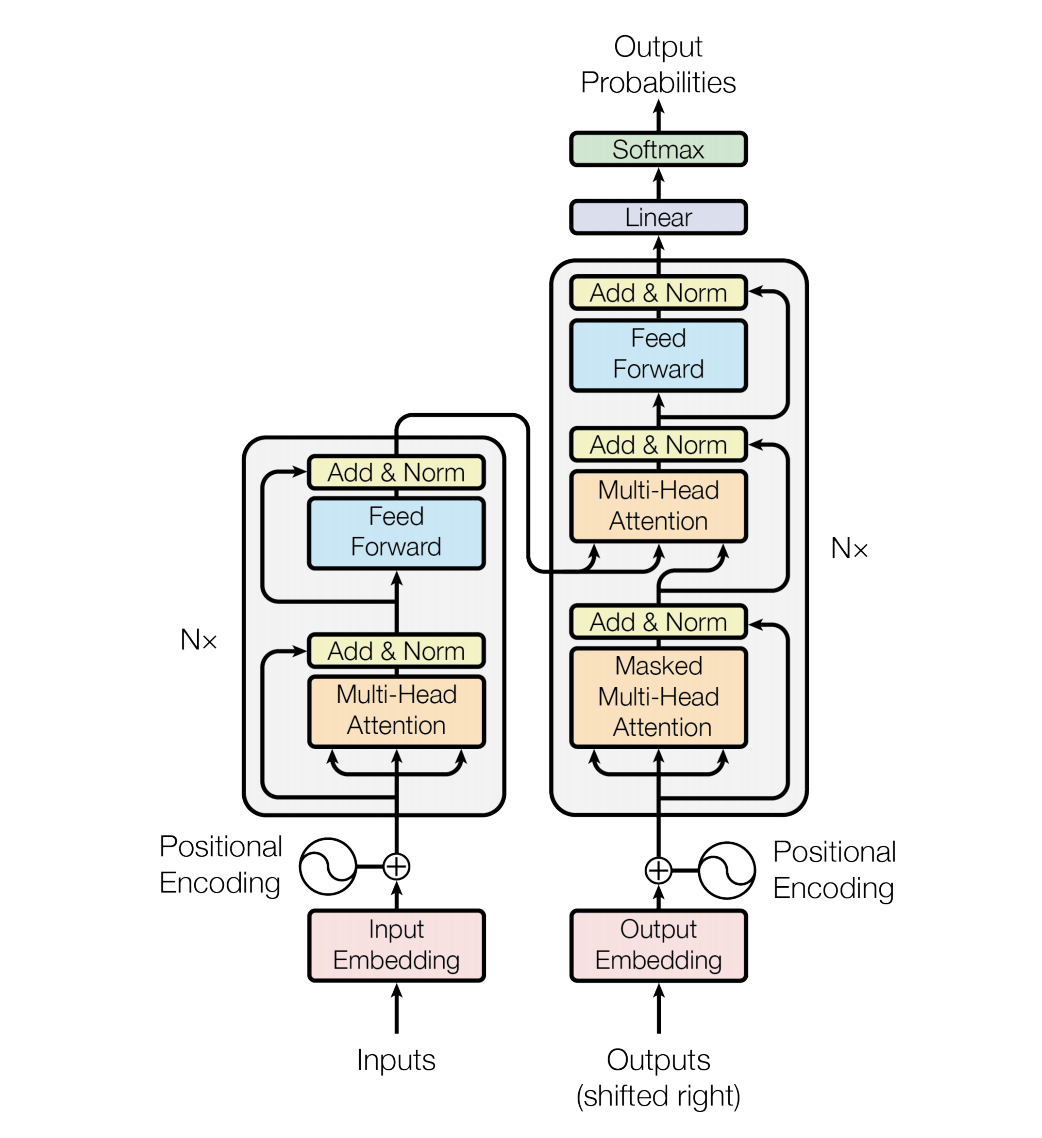
\includegraphics[height=0.5\textheight]{img/transformer}
        \caption[Original Transformer Architecture]{\textbf{Original Transformer Architecture.}
        The architecture was originally conceptualized for translation between languages.
        For that effect the text to translate (input) will be fully encoded to the embedding space, added to a positional encoding, and passed through alternating layers of self-attention and \gls{MLP} feed-forward layers with \gls{ReLU} activation, with residual connections and normalization after each.
        Output is generated autoregressively (generating each output token one-by-one, and append it to outputs to generate the next one), and has an additional layer of cross-attention to the input embedding.
        \Glspl{causal} are exclusively autoregressive decoder-only models.
        % The text to translate \textit{from} is the input, and the model will autoregressively (append selected output token to the outputs to generate the next output token until the full output has been generated) generate the full output.
        Image Source: \cite{vaswani_attention_2017}
        }
        \label{fig:transformer}
    \end{centering}
\end{figure}

% \begin{figure}[!htbp]
%     \begin{centering}
%         \subfloat[Runtime in minutes for correcting 25kb Matrix]
%         {\includegraphics[scale=0.9]{figures/results/runtime_25}} \\
%         % \caption[Correction time of 25kb]
%         % {\textbf{Runtime in minutes} for correcting the 25kb matrix.}
%         \subfloat[Runtime in minutes for correcting 50kb Matrix]
%         {\includegraphics[scale=0.9]{figures/results/runtime_50}}
%         \caption[Algorithm Runtimes]
%         {\textbf{Algorithm Runtimes} for correcting the different matrices. It
%         remains an open question why the difference between KR and RUST stays the
%         same, even though both ICE and RUST double their computation time. Smaller
%         is better.}
%         \label{fig:transformer}
%     \end{centering}
% \end{figure}


\subsection{The Transformer Architecture}\label{sub:transformer}
All modern language models are based on what Google introduced as the transformer architecture \cite{vaswani_attention_2017}. 
This architecture originally consisted of an encoder and a decoder (See \figref{transformer} for more details).
This new transformer architecture quickly established itself by outperforming other architectures available at the time with a fraction of the training cost.
An Encoder-Only transformer architecture, specifically \gls{BERT} set a new \gls{SOTA} for all \gls{NLP} benchmarks established at the time.
% This success was not limited to \gls{NLP} tasks.

% Along with significantly increasing capability in \acrlong{NLP}, these models enabled more sophisticated requests for data extraction.

% main difference to before: enabled more context compared to LSTM-based attention stuff (andscaling)

\subsection{A Modern Transformer Architecture}\label{sub:modern}

There have been various attempts at improving the transformer architecture \cite{shazeer_glu_2020, su_roformer_2022, ainslie_gqa_2023, bolya_hydra_2022, sukhbaatar_adaptive_2019, lu_understanding_2019, ye_understanding_2023, wu_memorizing_2022}, some of them more successful than others.
When setting up a new transformer model, there are a few established improvements that are used with few exceptions.
Compare with \figref{modern_transformer} for a graphic representation.

As activation functions, early transformer architectures used \gls{ReLU}, but when comparing different activation functions, \gls{SwiGLU} \cite{shazeer_glu_2020} empirically work best for most situations.

Instead of the previous sinusoidal positional encoding, using \gls{RoPE} works a lot better \cite{su_roformer_2022}. So does RMSNorm as LayerNorm \cite{ba_layer_2016}, when using it before instead of after each layer.

Grouping some of the query heads for \gls{GQA} \cite{ainslie_gqa_2023} work better than no sharing or full individual heads \cite{bolya_hydra_2022}.

\begin{figure}[!htbp]
    \begin{centering}
        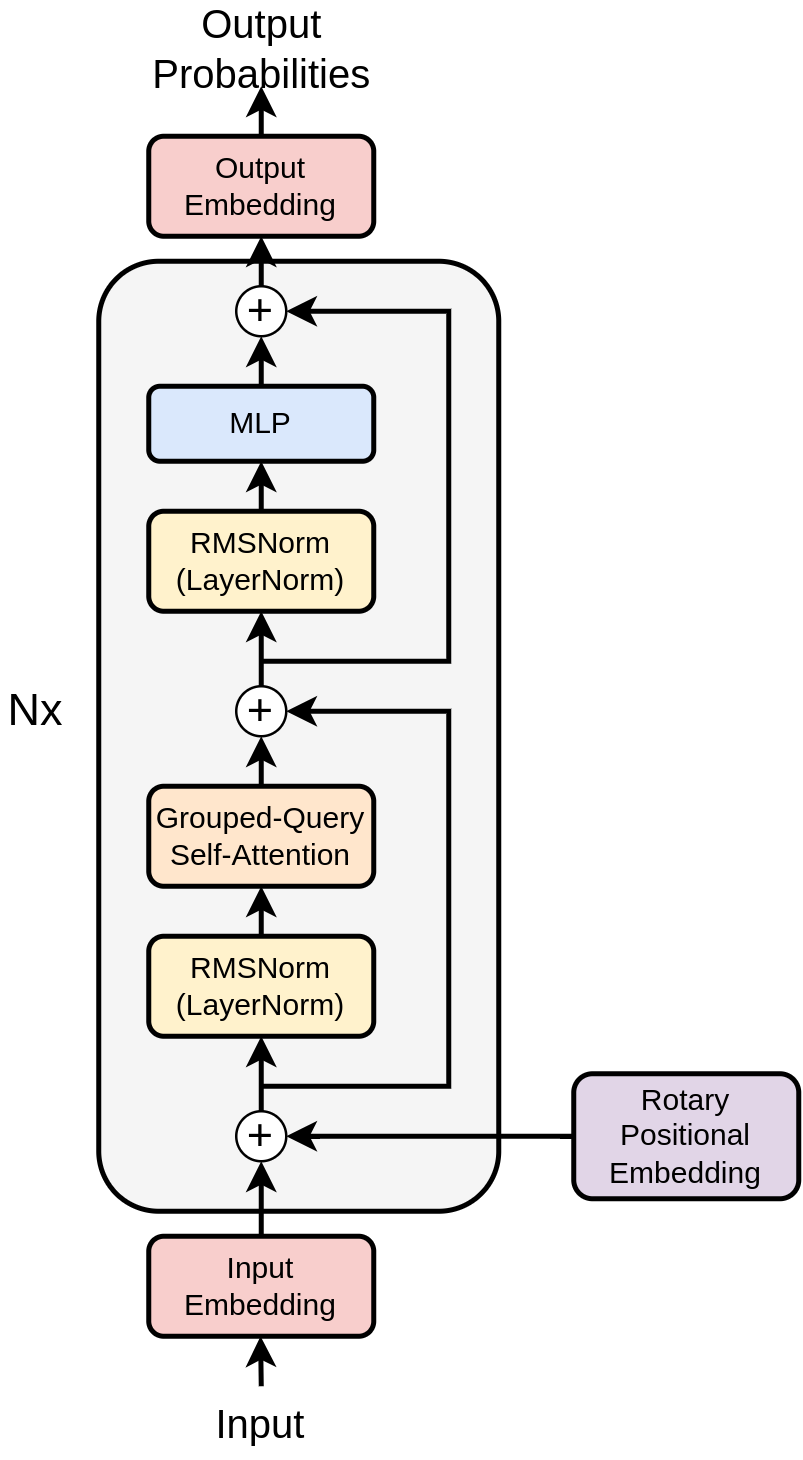
\includegraphics[height=0.8\textheight]{img/modern_transformer}
        \caption[Example of a Modern Transformer Architecture]{\textbf{Example of a Modern Transformer Architecture.} There are a number of differences when compared to the original architecture as seen previously in \figref{transformer}: layers are normalizing the residual with RMSNorm instead of having a normalized residual. Multi-head attention got replaced with \gls{GQA}, and sinusoidal positional embeddings with embeddings from \gls{RoPE} {\em on each layer}. Additionally, activation functions in the \gls{MLP} changed from \gls{ReLU} to \gls{SwiGLU}.}
        \label{fig:modern_transformer}
    \end{centering}
\end{figure}



This architecture, as described here and visualized in \figref{modern_transformer}, is shared with small variations by the \glspl{LLM} introduced later in \secref{models}.
Apart from \model{llama2}, most other \glspl{LLM} do not use \gls{GQA}.

Please refer to \cite{naveed_comprehensive_2023} for further details.

\subsection{Large Language Models}\label{sub:llm}

\gls{GPT2} \cite{radford_language_2019} is a very straightforward transformer architecture, but scaled up more than previous models.
The biggest \gls{GPT2} variant had 1.5 billion parameters, which is 15x more parameters than the biggest \gls{BERT} variant had.
It mainly demonstrated that bigger \glspl{LM} get more capable in general -- and seemingly without limit.

Models with more than a few billion parameters became generally referred to as a \acrlong{LLM}. \gls{GPT3}, the first such model with 176 billion parameters was introduced by \gls{OpenAI} in 2020 \cite{brown_language_2020}.
\glspl{LLM} differ from previous models in both parameter count (usually many billions) and substantial advances in general capability.
These models tend to have smaller siblings of the same architecture with fewer parameters, commonly in th steps of 7 billion, 13 billion, 30 billion, and 70 billion, though availability and exact parameter count varies.
Other Organisations trained \glspl{LLM} of this generation as well, some of them open-source, which demonstrated similar capabilities.
The most well-known models of this wave were \model{BLOOM} and \model{OPT} (throughout 2022).

The most recent and most capable generation of \glspl{LM} got introduced starting early 2023, after the release of \gls{ChatGPT} sparked worldwide interest in \glspl{LLM}. Progress happened fast and many incorporated numerous of the collectively found possible improvements. \glspl{LLM} of this generation are mostly classified so by their capability, and less so through parameter size, albeit their parameter counts still tend to be in the dozens of billions. Models of this category include the open-source \model{llama} and its well-known derivatives \model{alpaca} and \model{vicuna}, \model{falcon}, as well as most recently \model{llama2}.

For more details on most of the aforementioned models, see \secref{models}.


\section{Training Large Language Models}\label{sec:training}
\todo{write overeview of training methods}
\todo{mhm ... not quite happy how this section turned out. We'll see}


\subsection{Pretraining}\label{sub:pretraining}
Fundamentally, the objective of a \gls{causal} is to predict the next token based on the current token sequence.
The prediction of one token thus only depends on previous tokens.
For such scenarios, the reward is modeled as the likelyhood of predicting the correct token in the sequence.

To do the training, a high-quality dataset is also needed, numerous of which are publicly available \cite{redpajamadata_2023}.
You can find more details on this and additional parameters such as batch size and large scale distributed training in \cite{tirumala_d4_2023}.

\subsection{Fine-Tuning}\label{sub:finetune}
Fine-tuning exploits \textit{transfer learning} by continuing to train (See the previous \subref{pretraining} for details on training in general) a previously \textit{pre-trained} model, usually with a lower training rate and on very specialized data \cite{gaddipati_comparative_2020}.
This allows \textit{transferring} previosly learned features to accomplish a different task by making small adaptations.

As such, most fine-tuning and its resulting models is highly specialized.

\subsection{Fine-Tuning on Instructions}\label{sub:instruct}
Pre-trained or task-specific fine-tuned  models have learned context dependent token sequence likelihoods.
This is useful for predicting the 'next' token on a wikipedia article or novel, but this does not make it easy to utilize the model in other ways.

Essentially, fine-tuning on instructions guides the output by shifting the learned context-dependent token sequence likelihoods, providing more control over model outputs.
This results in users having a preference for the outputs of smaller models, over substantially bigger models, when the smaller model has been instruction-finetuned \cite{ouyang_training_2022}, as it makes the model more 'useful' in a naive sense.
A model fine-tuned on  a instruction dataset is commonly referred to as a \textit{instruct}-variant.

You can find more information on instruction-finetuning in \cite{ouyang_training_2022, tirumala_d4_2023}.


% \subsection{RLHF}\label{sub:rlhf}
% learning preference policy to later fine-tune the large model on. basically lobotomization, as it drastically reduces capability.
% Well, write it a bit nicer than that.
% \todo{this is not really relevant for my thesis. remove? or write?}
